
\section{Thursday}\index{week5_Thursday_lecture}
\subsection{Orthogonality}
Recall that two vectors are orthogonal if their inner product is zero:
\[
\bm u\perp\bm v
\Longleftrightarrow
\inp{\bm u}{\bm v}=0
\]

Orthogonality among vectors has an important property:
\begin{proposition}
If \emph{nonzero} vectors $v_1,\dots,v_k$ are mutually orthogonal, i.e., $v_i\perp v_j$ for any $i\ne j$, then $\{v_1,\dots,v_k\}$ must be ind.
\end{proposition}
\begin{proof}
It suffices to show that 
\[
\alpha_1v_1+\dots+\alpha_kv_k=\bm 0 \implies
\alpha_i=0\text{ for any $i\in\{1,2,\dots,k\}$.}
\]
\begin{itemize}
\item
We do inner product to show $\alpha_1$ must be zero:
\[
\begin{aligned}
\inp{v_1}{\alpha_1v_1+\dots+\alpha_kv_k}
&=\inp{v_1}{\bm 0}=0\\
&=\alpha_1\inp{v_1}{v_1}+\alpha_2\inp{v_1}{v_2}+\dots+\alpha_k\inp{v_1}{v_k}\\
&=\alpha_1\inp{v_1}{v_1}=\alpha_1\|v_1\|_2^2\\
&=0
\end{aligned}
\]
Since $v_1\ne \bm 0$, we have $\alpha_1=0$.
\item
Similarly, we have $\alpha_i=0$ for $i=1,\dots,k$.
\end{itemize}
\end{proof}
Now we can also talk about orthogonality among spaces:
\begin{definition}[Subspace Orthogonality]
Two subspaces $\bm U$ and $\bm V$ of a vector space are \emph{orthogonal} if every vector $\bm u$ in $\bm U$ is \textit{perpendicular} to every vector $\bm v$ in $\bm V$:
\[
\begin{array}{lll}
\mbox{\emph{Orthogonal subspaces}}
&
\bm u\perp\bm v,
&
\forall\bm u\in\bm U,\bm v\in\bm V.
\end{array}
\]
\end{definition}
\begin{example}
Two walls look \textit{perpendicular} but they are not orthogonal subspaces! The meeting line is in both $\bm U$ and $\bm V$-and this line is not perpendicular to itself. Hence, two planes (both with dimension $2$ in $\mathbb{R}^{3}$) cannot be orthogonal subspaces.

\begin{figure}[H]
\centering
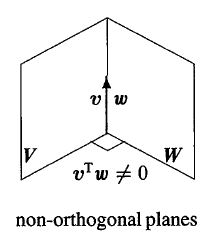
\includegraphics{week5/orthogonality}
\caption{Orthogonality is impossible when $\dim\bm U+\dim\bm V>\dim(\bm U\cup\bm V)$}
\end{figure}
\end{example}
\begin{remark}
When a vector is in two orthogonal subspaces, it \textit{must} be zero. It is \emph{perpendicular} to
itself. 
\\The reason is clear: this vector $\bm u\in\bm U$ and $\bm u\in\bm V$, so $\inp{\bm u}{\bm u}=0$. It has to be zero vector.
\end{remark}
If two subspaces are perpendicular, their basis must be ind.
\begin{theorem}
Assume $\{u_1,\dots,u_k\}$ is the basis for $\bm U$, $\{v_1,\dots,v_l\}$ is the basis for $\bm V.$ If $\bm U\perp\bm V$ ($u_i\perp v_j$ for $\forall i,j$), then $u_1,u_2,\dots,u_k,v_1,v_2,\dots,v_l$ must be ind.
\end{theorem}
\begin{proof}
Suppose there exists $\{\alpha_1,\dots,\alpha_k\}$ and $\{\beta_1,\dots,\beta_l\}$ such that
\[
\alpha_1u_1+\dots+\alpha_ku_k+\beta_1v_1+\dots+\beta_lv_l=\bm 0
\]
then equivalently,
\[
\alpha_1u_1+\dots+\alpha_ku_k=-(\beta_1v_1+\dots+\beta_lv_l).
\]
Then we set $\bm w=\alpha_1u_1+\dots+\alpha_ku_k$, obviously, $\bm w\in\bm U$ and $\bm w\in\bm V$.

 Hence it must be zero (This is due to remark above). Thus we have
\begin{gather*}
\alpha_1u_1+\dots+\alpha_ku_k=\bm 0\\
\beta_1v_1+\dots+\beta_lv_l=\bm 0.
\end{gather*}
Due to the independence, we have $\alpha_i=0$ and $\beta_j=0$ for $\forall i,j$. 
\end{proof}
\begin{corollary}
For subspaces $\bm U$ and $\bm V$, we obtain
\[
\dim(\bm U\cup\bm V)\le \dim(\bm U) + \dim(\bm V).
\]
\end{corollary}
For subspaces $\bm U$ and $\bm V\in\mathbb{R}^{n}$, if $\mathbb{R}^{n}=\bm U\cup\bm V$, and moreover, $n=\dim(\bm U)+\dim(\bm V)$, then we say $\bm V$ is the \emph{orthogonal complement} of $\bm U$.
\begin{definition}[orthogonal complement]
For subspaces $\bm U$ and $\bm V\in\mathbb{R}^{n}$, if $\dim(\bm U)+\dim(\bm V)=n$ and $\bm U\perp\bm V$, then we say $\bm V$ is the \emph{orthogonal complement} of $\bm U$. We denote $\bm V$ as $\bm U^{\perp}$.

Moreover, $\bm V=\bm U^{\perp}$ iff $\bm V^{\perp}=\bm U$.
\end{definition}
\begin{example}
Suppose $\bm U\cup\bm V=\mathbb{R}^{3}$, $\bm U=\Span\{\bm e_1,\bm e_2\}$. If $\bm V$ is the orthogonal complement of $\bm U$, then $\bm V=\Span\{\bm e_3\}$.
\end{example}

Next we study the relationship between the null space and the row space in $\mathbb{R}^n$.
\begin{theorem}[Fundamental theorem for linear alegbra, part 2] Given $\bm A\in\mathbb{R}^{m\times n}$,

\emph{$N(\bm A)$ is the orthogonal complement of the row space of $\bm A$, $\mathcal{C}(\bm A\trans)$ (in $\mathbb{R}^{n}$).}

\emph{$N(\bm A\trans)$ is the orthogonal complement of the column space $\mathcal{C}(\bm A)$ (in $\mathbb{R}^{m}$).}
\end{theorem}
\begin{proof}
\begin{itemize}
\item
Firstly, we show $\dim(N(\bm A))+\dim(\mathcal{C}(\bm A\trans))=n$:

We know that $\dim(N(\bm A))=n-r$ and $\dim(\mathcal{C}(\bm A\trans)) = r$, where $r=\rank(\bm A)$.

Hence $\dim(N(\bm A))+\dim(\mathcal{C}(\bm A\trans))=n$.
\item
Then we show $N(\bm A)\perp \mathcal{C}(\bm A\trans)$:

For any $x\in N(\bm A)$, if we set $\bm A=\begin{bmatrix}
a_1\trans\\a_2\trans\\\vdots\\a_m\trans
\end{bmatrix}$, then we obtain:
\[
\bm{Ax}=\begin{bmatrix}
a_1\trans\\a_2\trans\\\vdots\\a_m\trans
\end{bmatrix}\begin{bmatrix}
\bm x
\end{bmatrix}=\begin{bmatrix}
0\\0\\\vdots\\0
\end{bmatrix}
\]
Hence \textit{every row has a zero product with} $\bm x$, i.e., $\inp{a_i}{\bm x}=0$ for $\forall i\in\{1,2,\dots,m\}$.

For any $y=\sum_{i=1}^m\alpha_ia_i\in \mathcal{C}	(\bm A\trans)$, we obtain:
\[
\begin{aligned}
\inp{\bm x}{y}&=\inp{y}{\bm x}=\inp{\sum_{i=1}^m\alpha_ia_i}{\bm x}\\
&=\sum_{i=1}^{m}\alpha_i\inp{a_i}{\bm x}=0.
\end{aligned}
\]
Hence $\bm x\perp y$ for $\forall \bm x\in N(\bm A)$ and $y\in \mathcal{C}(\bm A\trans)$.\\
\end{itemize}
Hence $N(\bm A)^{\perp}=\mathcal{C}(\bm A\trans)$. Similarly, we have $N(\bm A\trans)^{\perp}=\mathcal{C}(\bm A)$. 
\end{proof}

\begin{corollary}
$\bm{Ax}=\bm b$ is solvable if and only if $\bm y\trans\bm A=\bm 0$ implies $\bm y\trans\bm b$=0.
\end{corollary}
\begin{proof} The following statements are equivalent:
\begin{itemize}
\item
$\bm{Ax}=\bm b$ is solvable.
\item
$\bm b\in \mathcal{C}(\bm A)$.
\item
$\bm b\in N(\bm A\trans)^{\perp}$
\item
$\bm y\trans\bm b=0$ for $\forall y\in N(\bm A\trans)$
\item
Given $\bm y\trans\bm A=\bm 0$, i.e., $y\in N(\bm A\trans)$, it implies $\bm y\trans\bm b=0$.
\end{itemize}
\end{proof}
The \emph{Inverse Negative Proposition} is more commonly useful:
\begin{corollary}
$\bm{Ax}=\bm b$ has no solution if and  and only if $\exists \bm y$ s.t. $\bm y\trans\bm A=0$ and $\bm y\trans\bm b\ne 0$.
\end{corollary}
We could extend this corollary into general case:
\begin{remark}
\begin{theorem}\label{theorem_12.3}
$\bm{Ax}\ge\bm b$ has no solution if and only if $\exists \bm y\ge\bm 0$ such that $\bm y\trans\bm A=\bm 0$ and $\bm y\trans\bm b\ge \bm 0$.
\end{theorem}
$\bm y\trans\bm A=0$ requires that there exists one linear combination of the row space to be zero.

The complete proof for this theorem is not required in this course. We only show the necessity case.
\begin{proof}[Necessity case.]
Suppose $\exists \bm y\ge\bm 0$ such that $\bm y\trans\bm A=\bm 0$ and $\bm y\trans\bm b\ge \bm 0$. Assume there exists $x^{*}$ such that $\bm Ax^{*}\ge\bm b$. By postmultiplying $\bm y\trans$ we have 
\[\bm y\trans\bm Ax^{*}\ge\bm y\trans\bm b>\bm 0
\implies 
\bm 0>\bm 0.
\]
which is a contradiction!
\end{proof}
\end{remark}

\begin{example}
Given the system 
\begin{align}
x_1+x_2&\ge1\label{Eq:6:3}
\\
-x_1&\ge-1\label{Eq:6:4}
\\
-x_2&\ge2\label{Eq:6:5}
\end{align}
Eq.(\ref{Eq:6:3})$\x$1+Eq(\ref{Eq:6:4})$\x$1+Eq.(\ref{Eq:6:5})$\x$1 gives
\[
0\ge 2
\]
which is a contradiction!\\
So the key idea of theorem (\ref{theorem_12.3}) is to construct a linear combination of row space to let it become zero. If the right hand is larger than zero, then this system has no solution.
\end{example}
\begin{remark}
\begin{corollary}
If $\bm A=\bm A\trans$, then $N(\bm A\trans)^{\perp}=\mathcal{C}(A)=\mathcal{C}(\bm A\trans)=N(\bm A)$.
\end{corollary}
\begin{corollary}\label{corollary_12.5}
The system $\bm{Ax}=\bm b$ may not have a solution, but $\bm A\trans\bm A\bm x=\bm A\trans\bm b$ always have at least one solution for $\forall\bm b$.
\end{corollary}
\begin{proof}
Since $\bm A\trans\bm A$ is symmetric, we have $\mathcal{C}(\bm A\trans\bm A)=\mathcal{C}(\bm A\bm A\trans)$. Show by yourself that $\mathcal{C}(\bm A\bm A\trans)=\mathcal{C}(\bm A\trans)$, hence $\mathcal{C}(\bm A\trans\bm A)=\mathcal{C}(\bm A\trans)$.

For any vector $\bm b$, we have $\bm A\trans\bm b\in \mathcal{C}(\bm A\trans)\implies\bm A\trans\bm b\in \mathcal{C}(\bm A\trans\bm A)$, which means there exists a linear combination of the columns of $\bm A\trans\bm A$ that equals to $\bm b$.

Or equivalently, there exists a solution to $\bm A\trans\bm A\bm x=\bm A\trans\bm b$.
\end{proof}
\begin{corollary}\label{corollary_12.6}
$\bm A\trans\bm A$ is invertible if and only if $\bm A$ is full column rank, i.e., columns of $\bm A$ are ind.
\end{corollary}
\begin{proof}
We have shown that $C(\bm A\trans\bm A)=C(\bm A\trans)$.

Hence $C(\bm A\trans\bm A)^{\perp}=C(\bm A\trans)^{\perp}\implies N(\bm A\trans\bm A)=N(\bm A)$.

Thus, the following statements are equivalent:
\begin{itemize}
\item
$\bm A$ has ind. columns
\item
$N(\bm A)=\{\bm 0\}$
\item
$N(\bm A\trans\bm A)=\{\bm 0\}$
\item
$\bm A\trans\bm A$ is invertible.
\end{itemize}
\end{proof}
\end{remark}
\subsection{Least Squares Approximations}
The linear system $\bm{Ax}=\bm b$ often has no solution, if so, what should we do?

We cannot always get the error $\bm e=\bm b-\bm{Ax}$ down to zero, so we want to use \textit{least square method} to minimize the error. In other words, our goal is to
\[
\min_{\bm x\in\mathbb{R}^n}\bm e^2:=\min_{\bm x}\|\bm{Ax}-\bm b\|^2=\sum_{i=1}^{m}(a_i\trans\bm x-b_i)^2
\]
where $\bm A\in\mathbb{R}^{m\times n}$ and $\bm b\in\mathbb{R}^m$. The minimizer $\bm x$ is called the \emph{linear least squares solution}.

\subsubsection{Least Squares by Convex Optimization}
Firstly, you should know some basic calculus knowledge for matrix:
\paragraph{The Chian Rule} Given two vectors $f(x),g(x)$ of appropriate size,
\[
\frac{\partial(f\trans g)}{\partial x}=\frac{\partial f(x)}{\partial x}g(x)+\frac{\partial g(x)}{\partial x}f(x)
\]
\paragraph{Examples of Matrix Derivative}
\begin{align}
\frac{\partial(a\trans \bm x)}{\partial \bm x}&=a\\
\frac{\partial(a\trans \bm A\bm x)}{\partial \bm x}&=\frac{\partial((\bm A\trans a)\trans\bm x)}{\partial \bm x}=\bm A\trans a\\
\frac{\partial(\bm A\bm x)}{\partial \bm x}&=\bm A\trans\\
\frac{\partial(\bm x\trans\bm A\bm x)}{\partial \bm x}&=\bm A\bm x+\bm A\trans\bm x
\end{align}

Thus, in order to minimize $\|\bm{Ax}-\bm b\|^2=(\bm{Ax}-\bm b)\trans(\bm{Ax}-\bm b)$, it suffices to let its \emph{derivative} with respect to $\bm x$ to be \emph{zero.} (Since $\|\bm{Ax}-\bm b\|^2$ is convex, which will be discussed in detail in other courses.) Hence we have:
\[\begin{aligned}
\frac{\partial (\bm{Ax}-\bm b)\trans(\bm{Ax}-\bm b)}{\partial \bm x}&=\frac{\partial(\bm{Ax}-\bm b)}{\partial \bm x}(\bm{Ax}-\bm b)+\frac{\partial(\bm{Ax}-\bm b)}{\partial \bm x}(\bm{Ax}-\bm b)\\
&=2\frac{\partial(\bm{Ax}-\bm b)}{\partial \bm x}(\bm{Ax}-\bm b)\\
&=2(\frac{\partial(\bm A\bm x)}{\partial \bm x}-\frac{\partial(\bm b)}{\partial \bm x})(\bm{Ax}-\bm b)\\
&=2\bm A\trans(\bm{Ax}-\bm b)=\bm 0.
\end{aligned}
\]
Or equivalently, 
\[
\bm A\trans\bm{Ax}=\bm A\trans\bm b.
\]
According to corollary (\ref{corollary_12.5}), this equation always exists a solution. This equation is called the \emph{normal equation}.
\begin{theorem}\label{theorem_12.4}
A vector $\bm x_{\text{LS}}$ is an optimal solution to the least squares problem
\begin{subequations}
\begin{equation}
\min_{\bm x\in\mathbb{R}^n}\|\bm b-\bm{Ax}\|_2^2
\end{equation}
if and only if it satisfies
\begin{equation}
\bm A\trans\bm A\bm x_{\text{LS}} = \bm A\trans\bm b.
\end{equation}
\end{subequations}
\end{theorem}
\subsubsection{Fit a stright line}
Given a collection of data $(\bm x_i,y_i)$ for $i=1,\dots,m$, we can use a stright line to fit these points:
\[
\left\{
\begin{aligned}
y_1&=a_0+a_1x_{1,1}+a_2x_{1,2}+\dots+a_nx_{1,n}+\varepsilon_1\\
y_2&=a_0+a_1x_{2,1}+a_2x_{2,2}+\dots+a_nx_{2,n}+\varepsilon_2\\
\vdots\\
y_m&=a_0+a_1x_{m,1}+a_2x_{m,2}+\dots+a_nx_{m,n}+\varepsilon_m
\end{aligned}
\right.
\]
Our fit line is 
\[
\hat y=a_0+a_1x_1+a_2x_2+\dots+a_nx_n
\]
In \textit{compact matrix form}, we have
\[
\begin{bmatrix}
y_1\\y_2\\\vdots\\y_n
\end{bmatrix}
=\begin{bmatrix}
1&x_{1,1}&x_{1,2}&\dots&x_{1,n}\\
1&x_{2,1}&x_{2,2}&\dots&x_{2,n}\\
\vdots&\vdots&&&\\
1&x_{m,1}&x_{m,2}&\dots&x_{m,n}\\
\end{bmatrix}\begin{bmatrix}
a_0\\a_1\\a_2\\\vdots\\a_{n}
\end{bmatrix}+\begin{bmatrix}
\varepsilon_1\\\varepsilon_2\\\vdots\\\varepsilon_m
\end{bmatrix}
\]
Or equivalently, we have 
\[
\bm y=\bm{Ax}+\bm \varepsilon
\]
where $\bm A =\begin{bmatrix}
1&x_{1,1}&x_{1,2}&\dots&x_{1,n}\\
1&x_{2,1}&x_{2,2}&\dots&x_{2,n}\\
\vdots&\vdots&&&\\
1&x_{m,1}&x_{m,2}&\dots&x_{m,n}\\
\end{bmatrix}_{m\times (n+1)}$, $\bm x=\begin{bmatrix}
a_0\\a_1\\a_2\\\vdots\\a_{n}
\end{bmatrix}_{(n+1)\times 1}$, $\bm \varepsilon=\begin{bmatrix}
\varepsilon_1\\\varepsilon_2\\\vdots\\\varepsilon_m
\end{bmatrix}_{m\times 1}$.\\
Our goal is to minimize $\|\hat{\bm y}-\bm y\|^2=\|\bm{Ax}-\bm y\|^2$. Then by theorem (\ref{theorem_12.4}), it suffices to sovle $\bm A\trans\bm A\bm x=\bm A\trans\bm y$.

\subsection{Projections}
In corollary (\ref{corollary_12.6}), we know that if $\bm A$ has ind. columns, then $\bm A\trans\bm A$ is invertible. On this condition, the normal equation $\bm A\trans\bm A\bm x=\bm A\trans\bm b$ has the unique solution $\bm x^{*}=(\bm A\trans\bm A)^{-1}\bm A\trans\bm b$, which follows that the error $\bm b-\bm A\bm x^{*}$ is minimized. Note that $\bm A\bm x^{*}=\bm A(\bm A\trans\bm A)^{-1}\bm A\trans\bm b$ is \emph{approximately} equal to $\bm b$. 
\begin{itemize}
\item
If $\bm b$ and $\bm{A}\bm x^{*}$ are exactly in the same space, i.e., $\bm b\in\mathcal{C}(\bm A)$, then $\bm{A}\bm x^{*}=\bm b$. The error is equal to zero.
\item
Otherwise, just as the Figure (\ref{figure_12.2}) shown, $\bm A\bm x^{*}$ is the projection of $\bm b$ to subspace $\mathcal{C}(\bm A)$.
\end{itemize}
\begin{figure}[t]
\centering
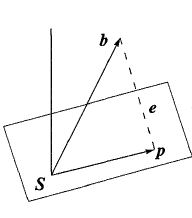
\includegraphics{week5/projection}
\caption{The projection of $\bm b$ onto a subspace $\bm S:=\mathcal{C}(\bm A)$.}\label{figure_12.2}
\end{figure}
\begin{definition}[Projection]
Let $\bm S\in\mathbb{R}^{m}$ be a non-empty closed set and $\bm b\in\mathbb{R}^m$ be given. Then the projection of $\bm b$ onto the set $\bm S$ is the solution to
\[
\min_{\bm z\in\bm S}\|\bm z-\bm b\|_2^2,
\]
where we use notation $\Proj_{\bm S}(\bm b)$ to denote the projection of $\bm b$ onto $\bm S$.
\end{definition}
By definition, the projection of $\bm b$ onto the subspace $\mathcal{C}(\bm A)$ is given by 
\[
\Proj_{\mathcal{C}(\bm A)}(\bm b):=\bm A\bm x^*,\quad
\text{where }\bm x^*=\arg\min_{\bm x\in\mathbb{R}^n}\|\bm{Ax} - \bm b\|.
\]

\begin{definition}[Projection matrix]
Given the projection
\[
\Proj_{C(\bm A)}(\bm b):=\bm A\bm x^{*}=\bm A(\bm A\trans\bm A)^{-1}\bm A\trans\bm b,
\]
since $[\bm A(\bm A\trans\bm A)^{-1}\bm A\trans]\bm b$,
we call the projection operator $\bm P:=\bm A(\bm A\trans\bm A)^{-1}\bm A\trans$ as the \emph{projection matrix} of $\bm A$.
\end{definition}
\begin{definition}[Idempotent]
Let $\bm A$ be a \emph{square} matrix that satisfies $\bm A=\bm A\bm A$, then $\bm A$ is called an \emph{idempotent} matrix.
\end{definition}
Let's show that the projection matrix is \textit{idempotent}:
\[
\begin{aligned}
\bm P^{2}&=\bm A(\bm A\trans\bm A)^{-1}\bm A\trans\bm A(\bm A\trans\bm A)^{-1}\bm A\trans\\
&=\bm A(\bm A\trans\bm A)^{-1}(\bm A\trans\bm A)(\bm A\trans\bm A)^{-1}\bm A\trans\\
&=\bm A(\bm A\trans\bm A)^{-1}\bm A\trans=\bm P.
\end{aligned}
\]

\subsubsection{Observations}
\begin{itemize}
\item
Suppose $\bm b\in \mathcal{C}(\bm A)$, i.e., $\exists \bm x$ s.t. $\bm{Ax}=\bm b$. Then the projection of $\bm b$ is exactly $\bm b$:
\[
\begin{aligned}
\bm{Pb}&=\bm A(\bm A\trans\bm A)^{-1}\bm A\trans(\bm b)\\
&=\bm A(\bm A\trans\bm A)^{-1}\bm A\trans(\bm{Ax})\\
&=\bm A(\bm A\trans\bm A)^{-1}(\bm A\trans\bm A)\bm x\\
&=\bm{Ax}=\bm b.
\end{aligned}
\]
\item
Assume $\bm A$ has only one column, say, $\bm a$. Then we have
\[\begin{aligned}
\bm x^{*}&=(\bm A\trans\bm A)^{-1}\bm A\trans\bm b=\frac{\bm a\trans\bm b}{\bm a\trans\bm a}\\
\bm A\bm x^{*}&=\bm{Pb}=\bm A(\bm A\trans\bm A)^{-1}\bm A\trans(\bm b)=\frac{\bm a\trans\bm b}{\bm a\trans\bm a}\times\bm a=\frac{\bm a\trans\bm b}{\|\bm a\|^2}\times\bm a
\end{aligned}
\]
More interestingly, 
\[\frac{\bm a\trans\bm b}{\|\bm a\|^2}\times\bm a=\frac{\|\bm a\|\|\bm b\|\cos\theta}{\|\bm a\|^2}\times\bm a=\|\bm b\|\cos\theta\times\frac{\bm a}{\|\bm a\|}\]
which is the projection of $\bm b$ onto a line $\Span\{\bm a\}$. (Shown in figure (\ref{Fig:6:3}).)
\begin{figure}[H]
\centering
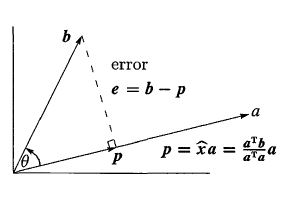
\includegraphics[width=10cm]{week5/projection_line}
\caption{The projection of $\bm b$ onto a line $\bm a$.}
\label{Fig:6:3}
\end{figure}
More generally, we can write the projection of $\bm b$ onto the line $\Span\{\bm a\}$ as:
\[
\Proj_{\Span\{\bm a\}}(\bm b)=\frac{\inp{\bm a}{\bm b}}{\inp{\bm a}{\bm a}}\bm a
\]
\paragraph{Changing an Orthogonal Basis}
Note that the error $\bm b-\Proj_{\Span\{\bm a\}}(\bm b)$ is perpendicular to $\bm a$, and $\bm b-\Proj_{\Span\{\bm a\}}(\bm b)\in\Span\{\bm a,\bm b\}.$

If we define $\bm b'=\bm b-\Proj_{\Span\{\bm a\}}(\bm b)$, then it's easy to check that $\Span\{\bm a,\bm b'\}=\Span\{\bm a,\bm b\}$ and $\bm a\perp\bm b'$. 

Hence, we convert the basis $\{\bm a,\bm b\}$ into another basis $\{\bm a,\bm b'\}$ such that the elements are orthogonal to each other. For general subspace we could also use this approach to obtain an orthogonal basis, which will be discussed in next lecture. 
\end{itemize}








